\documentclass[12pt]{article}
\usepackage{graphicx}
\usepackage{subcaption}
\usepackage{mwe}
\usepackage[]{mcode}
%\usepackage{lingmacros}
%\usepackage{tree-dvips}
%\usepackage{blindtext}
%\usepackage[utf8]{inputenc}

\begin{document}

\title{CMSC 426 - P1}
\author{Gudjon Einar Magnusson}

\maketitle

\section{Gaussian Filter Bank}

The Gaussian derivative filter is generated by first creating a simple Gaussian filter an then get the derivative by running a Sobel filter on it. The pixel size of the filter is defined to be $2\lceil sigma \times 3 \rceil + 1$.

For my filter bank I generated 24 different versions, 8 orientations and 3 scales, $sigma = \{1, 2, 4\}$.

\begin{figure}
    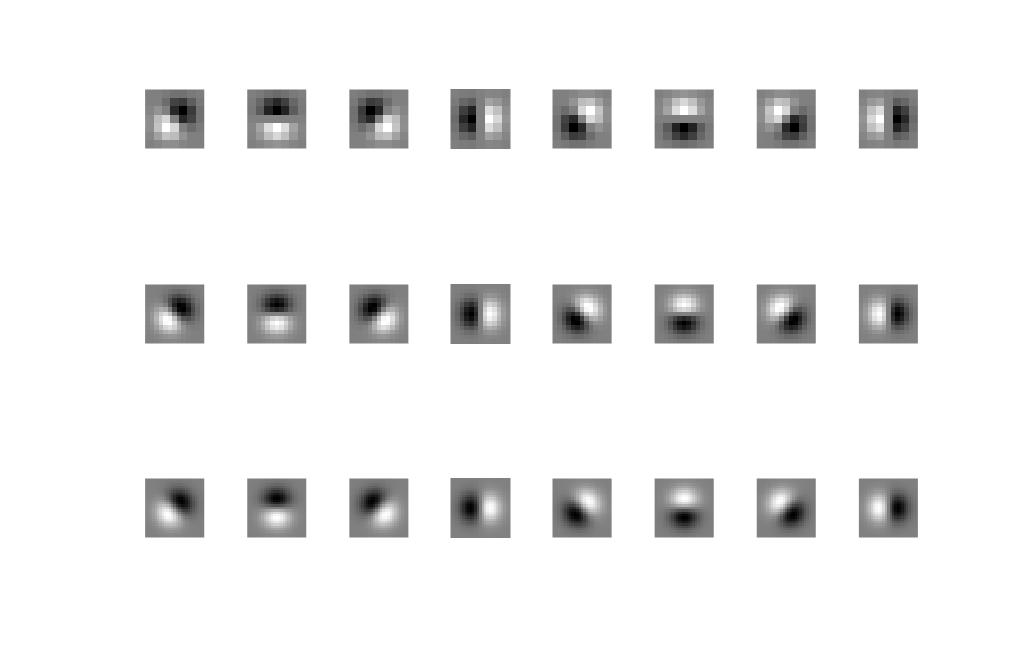
\includegraphics[width=\linewidth]{img/gfbank}
    \caption{Gaussian Filter Bank}
    \label{fig_gfbank}
\end{figure}


\section{Half-disk Masks}

To generate a half-disk with radius $r$ I first generate square matrix of size $2\lceil r \rceil +1$. Cells that have a square distance from the center less than $r^2$ get a value of $1$ others are $0$. Next I give every cell with a row index greater than $\lceil r \rceil +1$ a value of $0$. To rotate the half-disk I used the Matlab function \textit{imrotate}.

For my mask bank I chose to use 8 different orientations and 3 different radii, $r = \{2.8, 4.8, 6.8\}$. I found that using a radius that is a fraction instead of a whole number produces a cleaner looking circle.

\begin{figure}
    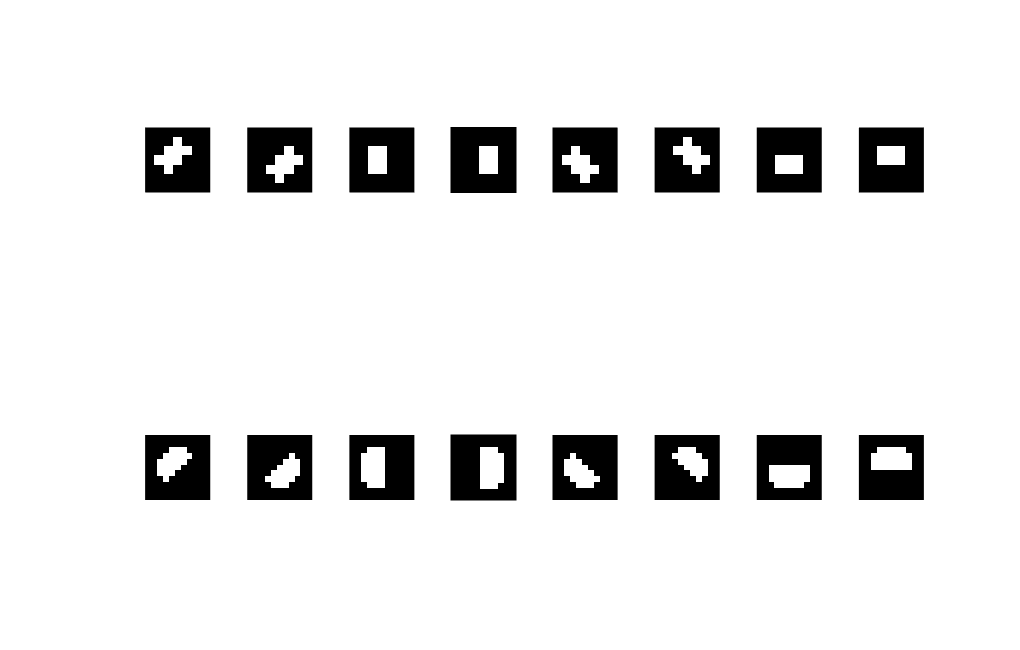
\includegraphics[width=\linewidth]{img/hdbank}
    \caption{Half-disk Masks}
    \label{fig_hdbank}
\end{figure}


\section{Image Gradients}

I generate gradient maps by first generating version of the image that emphases specific features and the comparing the histogram of values surrounding each pixel.

In my implementation I combine 3 different gradients, texture gradient, brightness gradient and color gradient. 

\subsection{Texture Gradient}

The texton map is generated by first filtering the image with each of the Gaussian filters and then running kmeans on the result. I chose to use 16 clusters for for the texton map.

\begin{figure}
    \begin{subfigure}[t]{.49\textwidth}
        \centering
        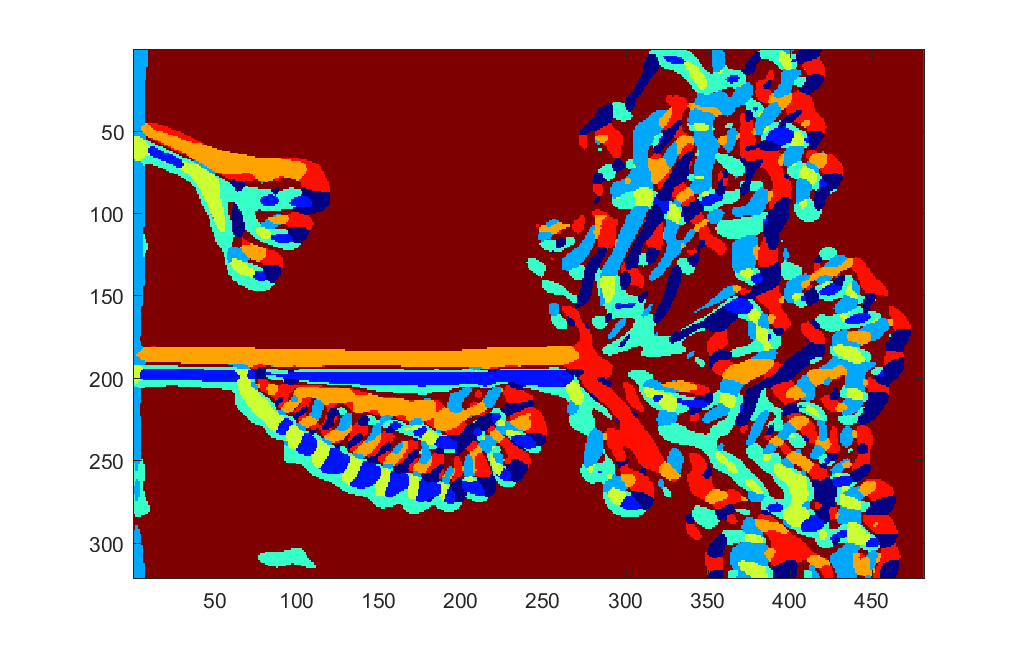
\includegraphics[width=\linewidth]{img/tmap1}
        \caption{Texton map}
        \label{fig_bmap1}
    \end{subfigure}\hfill
    \begin{subfigure}[t]{.49\textwidth}
        \centering
        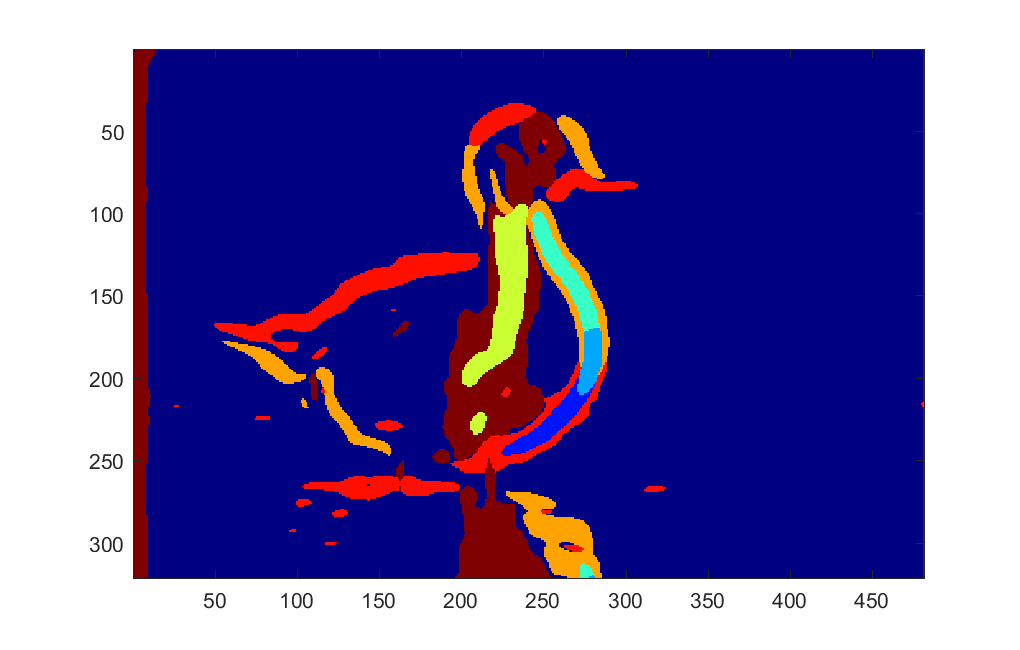
\includegraphics[width=\linewidth]{img/tmap2}
        \caption{Texton map}
        \label{fig_bmap2}
    \end{subfigure}

    \vskip\baselineskip

    \begin{subfigure}[t]{.49\textwidth}
        \centering
        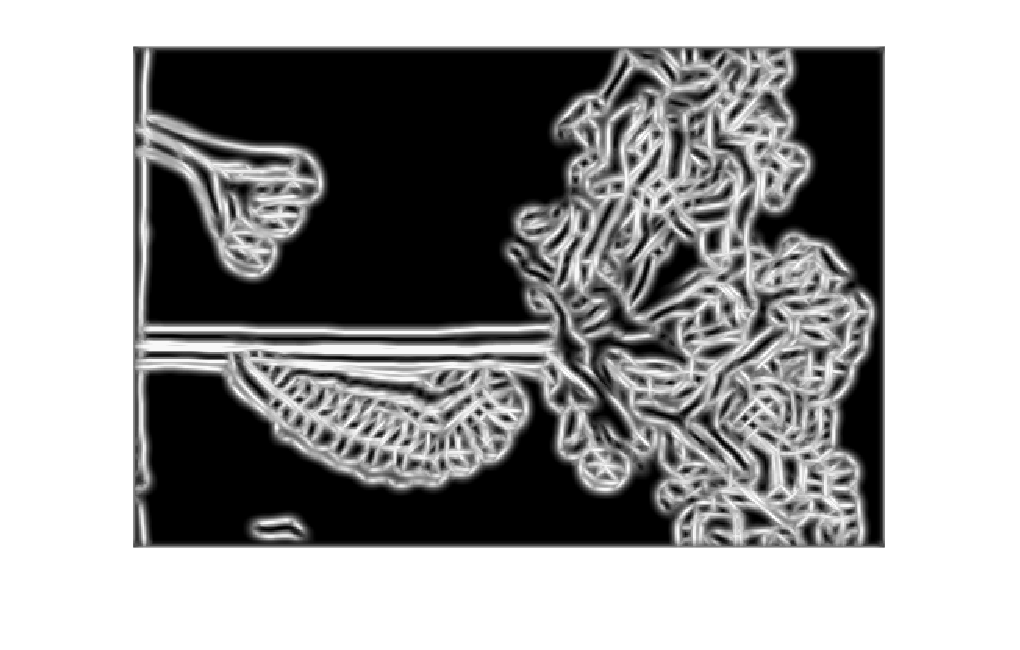
\includegraphics[width=\linewidth]{img/tg1}
        \caption{Texture gradient}
    \end{subfigure}\hfill
    \begin{subfigure}[t]{.49\textwidth}
        \centering
        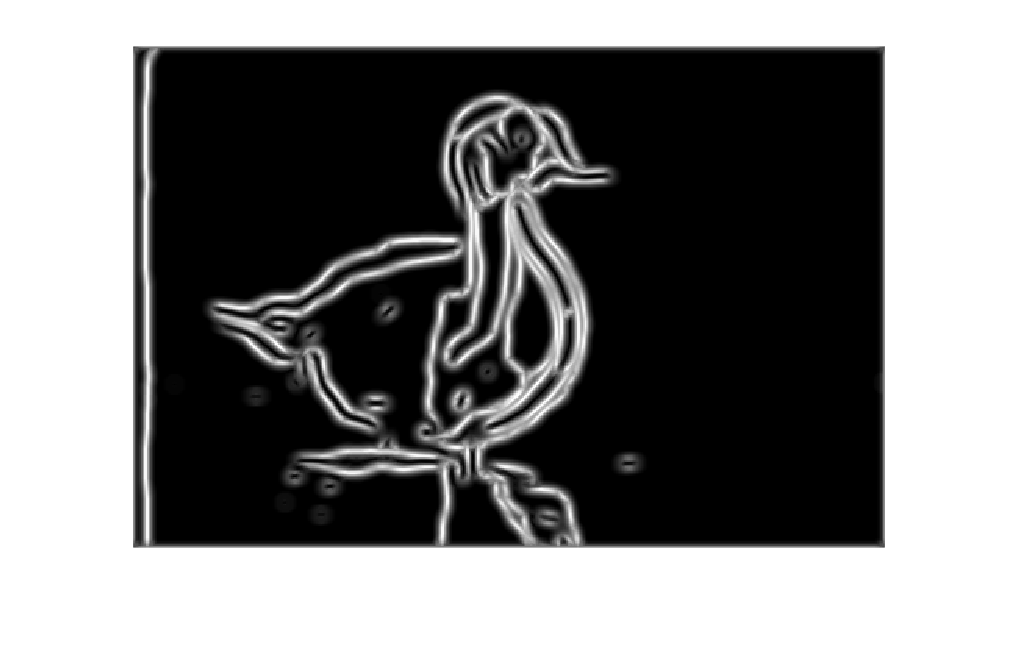
\includegraphics[width=\linewidth]{img/tg2}
        \caption{Texture gradient}
    \end{subfigure}
    \caption{Texton map and the resulting texture gradient}
    \label{fig_bg}
\end{figure}

\subsection{Brightness Gradient}

A brightness map is generated by grouping pixels based on the luminance value in the Lab color space. To do this I normalize the values in Lab color space to $0-1$ range, multiply by the number of groups and round up. I chose to use 32 groups for the brightness map. As you can see in figure \ref{fig_bmap1} an \ref{fig_bmap2}, sometimes this produces a nice separation between objects, but sometimes it does not.


\begin{figure}
    \begin{subfigure}[t]{.49\textwidth}
        \centering
        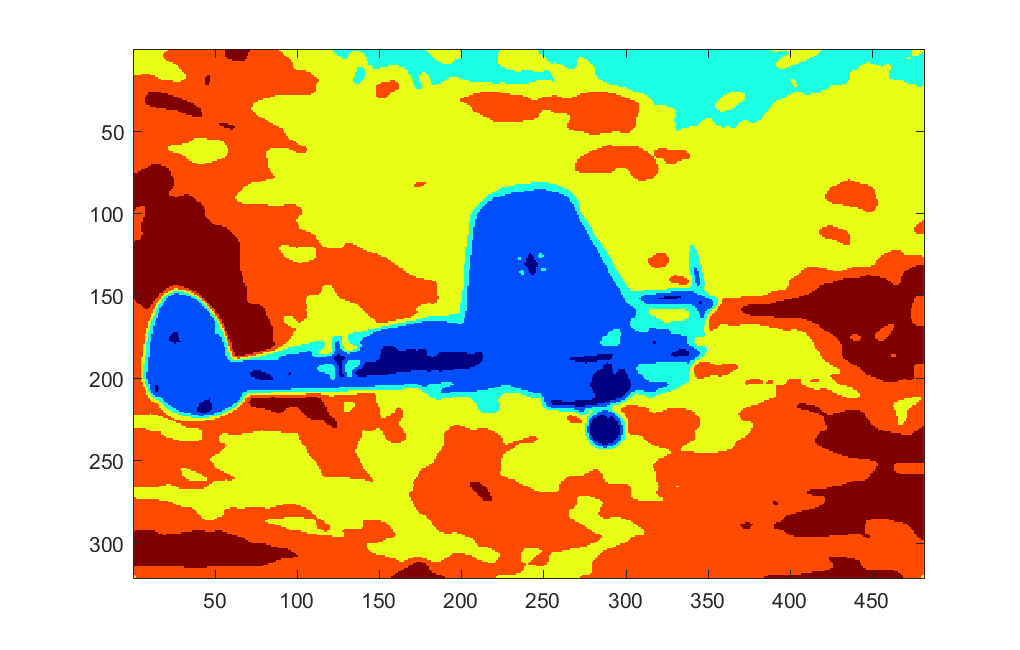
\includegraphics[width=\linewidth]{img/bmap1}
        \caption{Brightness map}
        \label{fig_bmap1}
    \end{subfigure}\hfill
    \begin{subfigure}[t]{.49\textwidth}
        \centering
        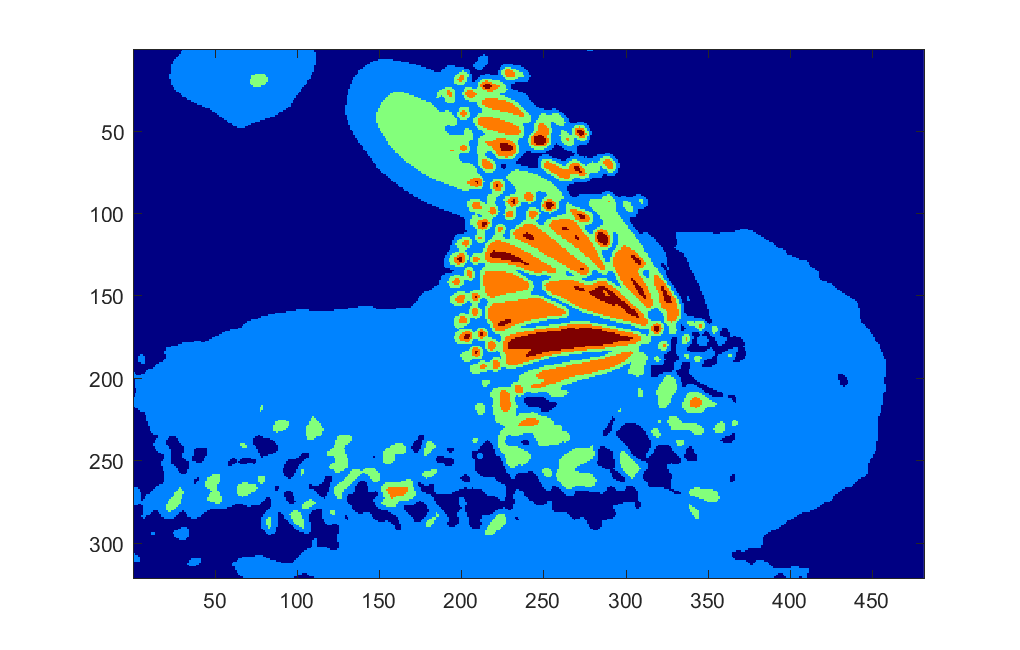
\includegraphics[width=\linewidth]{img/bmap2}
        \caption{Brightness map}
        \label{fig_bmap2}
    \end{subfigure}

    \vskip\baselineskip

    \begin{subfigure}[t]{.49\textwidth}
        \centering
        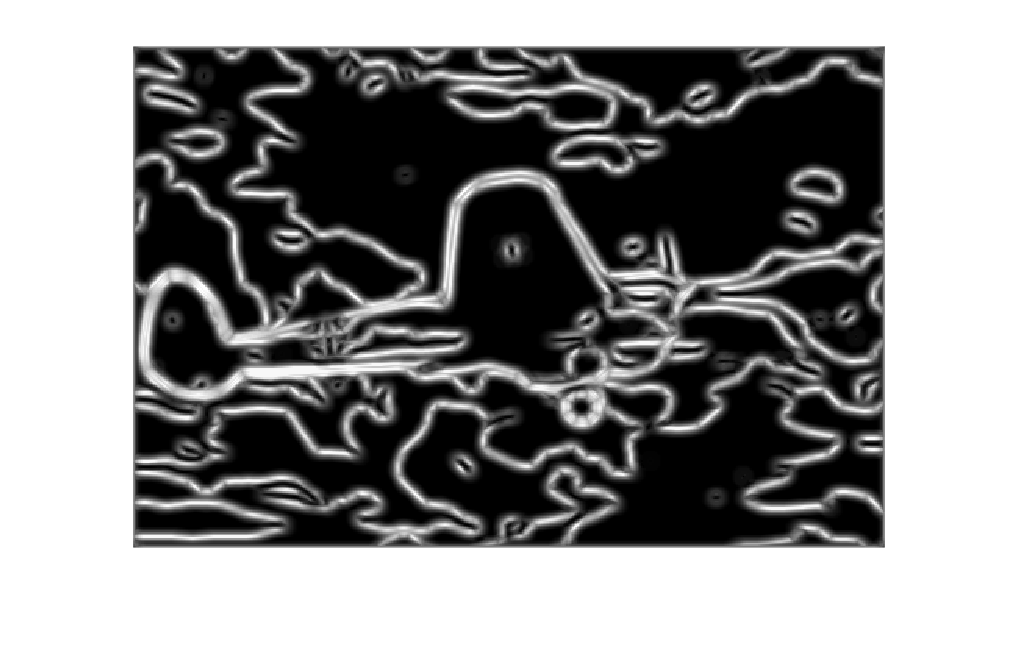
\includegraphics[width=\linewidth]{img/bg1}
        \caption{Brightness gradient}
    \end{subfigure}\hfill
    \begin{subfigure}[t]{.49\textwidth}
        \centering
        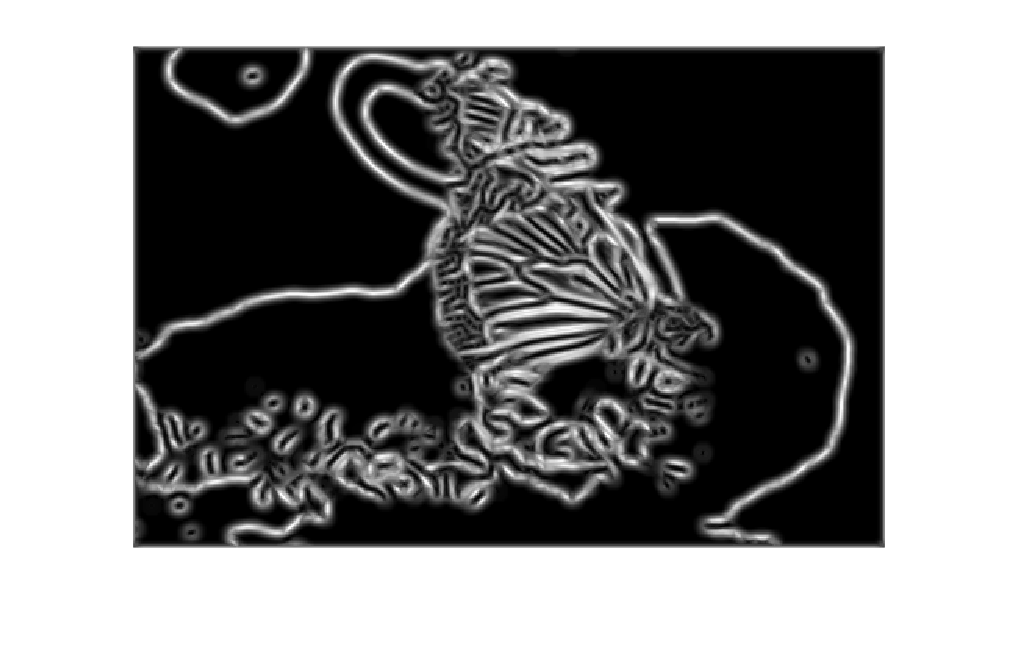
\includegraphics[width=\linewidth]{img/bg2}
        \caption{Brightness gradient}
    \end{subfigure}
    \caption{Brightness map and the resulting brightness gradient}
    \label{fig_bg}
\end{figure}


\subsection{Color Gradient}

To generate a color map I run kmeans on the a ans b channels of the Lab color space. Since the Lab color space is specially designed to make colors that are visually close have a small euclidean distance, kmeans should be able produce meaningful color clusters.

\begin{figure}
    \begin{subfigure}[t]{.49\textwidth}
        \centering
        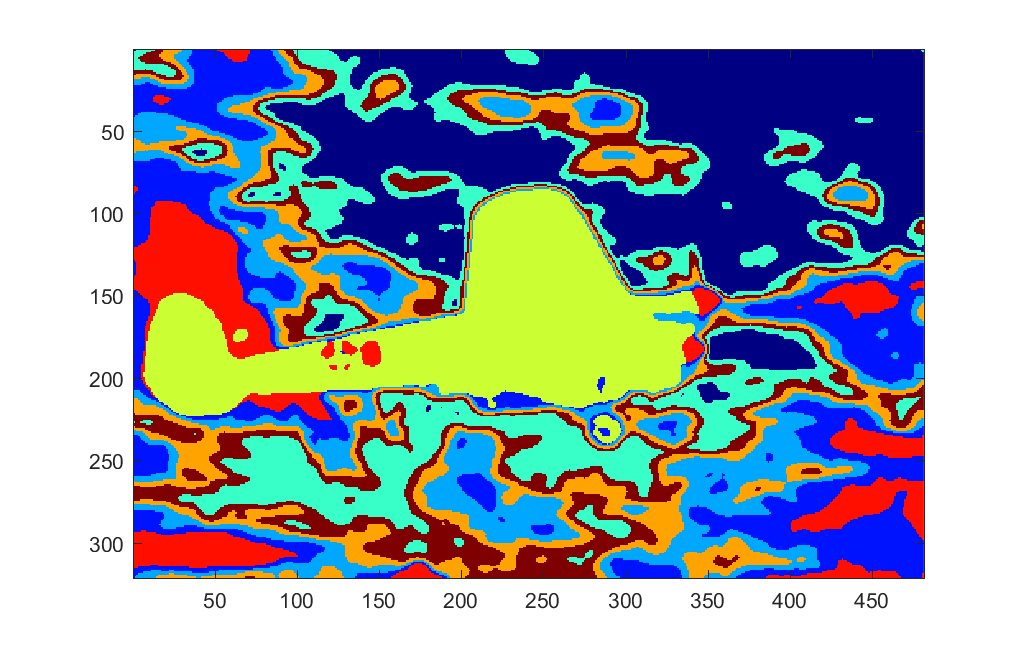
\includegraphics[width=\linewidth]{img/cmap1}
        \caption{Color map}
        \label{fig_bmap1}
    \end{subfigure}\hfill
    \begin{subfigure}[t]{.49\textwidth}
        \centering
        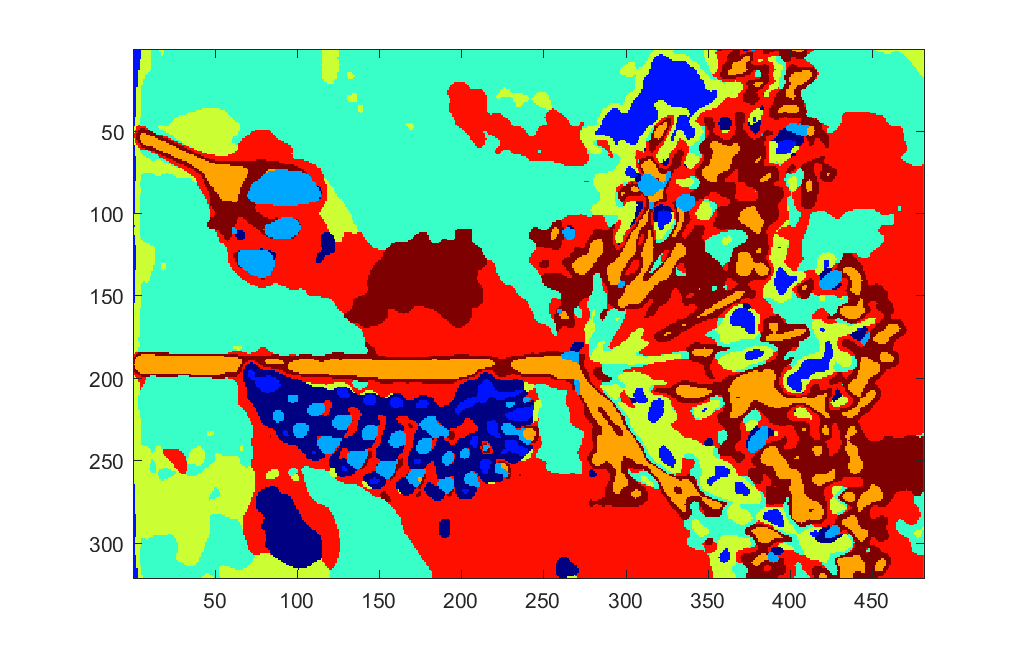
\includegraphics[width=\linewidth]{img/cmap2}
        \caption{Color map}
        \label{fig_bmap2}
    \end{subfigure}

    \vskip\baselineskip

    \begin{subfigure}[t]{.49\textwidth}
        \centering
        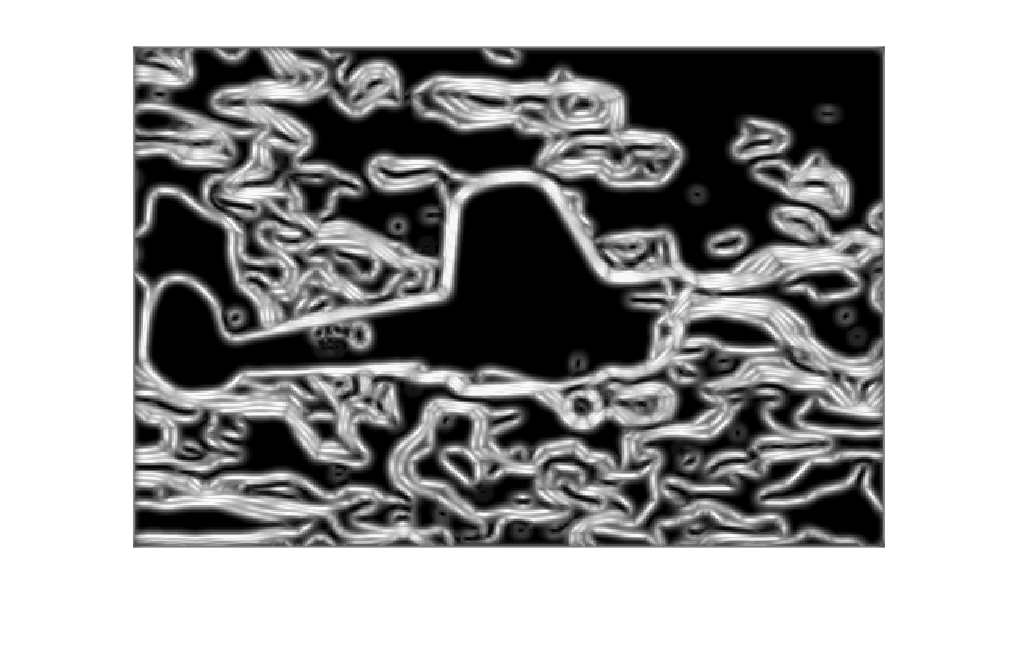
\includegraphics[width=\linewidth]{img/cg1}
        \caption{Brightness gradient}
    \end{subfigure}\hfill
    \begin{subfigure}[t]{.49\textwidth}
        \centering
        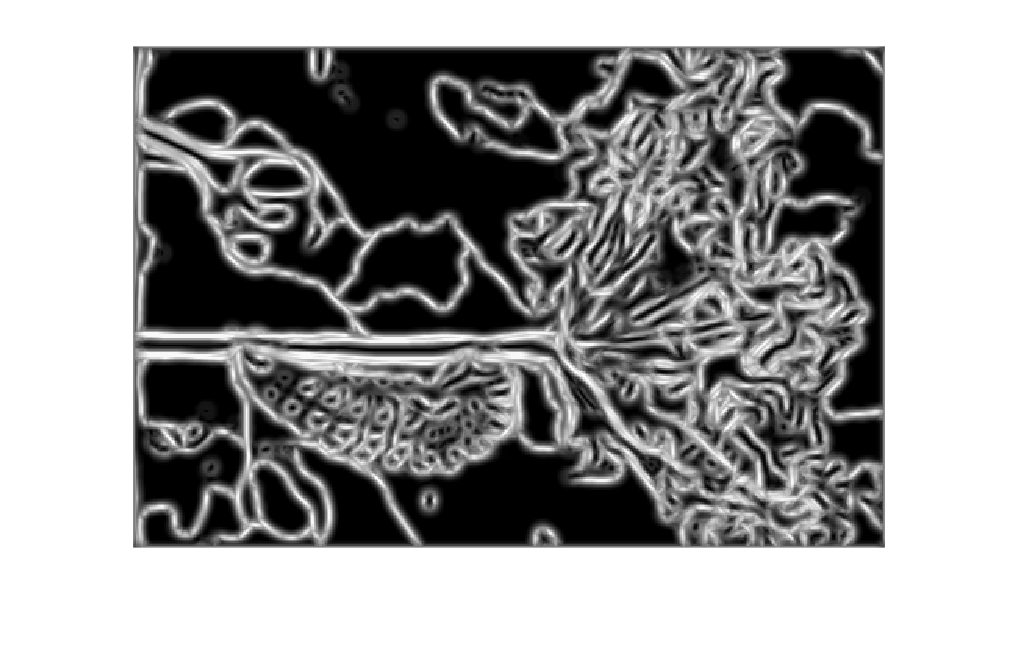
\includegraphics[width=\linewidth]{img/cg2}
        \caption{Brightness gradient}
    \end{subfigure}
    \caption{Brightness map and the resulting brightness gradient}
    \label{fig_bg}
\end{figure}

\section{Results}

Tweaking the size of the half-disk masks and picking a good cluster number for each of the maps turned out to be very difficult. I needed large half-disk to the be able to generalize textures that repeat over a large area but that makes the outlines very thick and fuzzy, which brings down the precision.

My strategy was to use low cluster numbers to find large flat clusters and small half-disks to try to find sharp edges. Large clusters causes each of the gradient maps to lose some edges but between all of them they usually find all the important edges. 

In the my edges ended up being very fizzy and with a lot of noise around them. My multiplying my results with the canny base line I get cleaner results but the PR curve does not look much better than with just canny.

\begin{figure}
    \begin{subfigure}[t]{.49\textwidth}
        \centering
        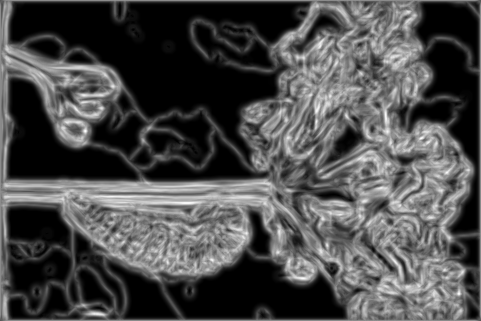
\includegraphics[width=\linewidth]{img/mypb1}
        \caption{Color map}
        \label{fig_bmap1}
    \end{subfigure}\hfill
    \begin{subfigure}[t]{.49\textwidth}
        \centering
        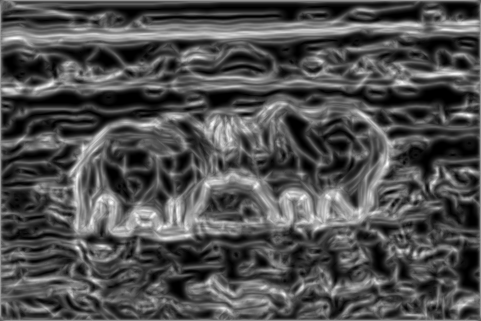
\includegraphics[width=\linewidth]{img/mypb2}
        \caption{Color map}
        \label{fig_bmap2}
    \end{subfigure}

    \vskip\baselineskip

    \begin{subfigure}[t]{.49\textwidth}
        \centering
        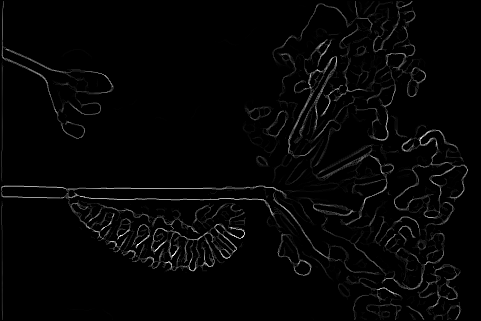
\includegraphics[width=\linewidth]{img/pblite1}
        \caption{Brightness gradient}
    \end{subfigure}\hfill
    \begin{subfigure}[t]{.49\textwidth}
        \centering
        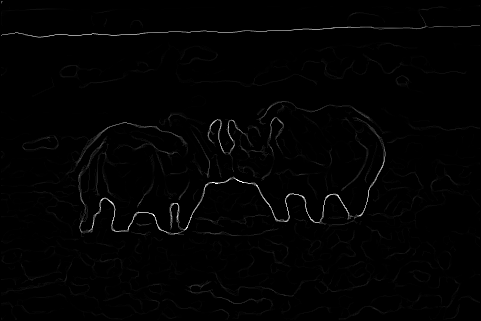
\includegraphics[width=\linewidth]{img/pblite2}
        \caption{Brightness gradient}
    \end{subfigure}
    \caption{Brightness map and the resulting brightness gradient}
    \label{fig_bg}
\end{figure}

\begin{figure}
    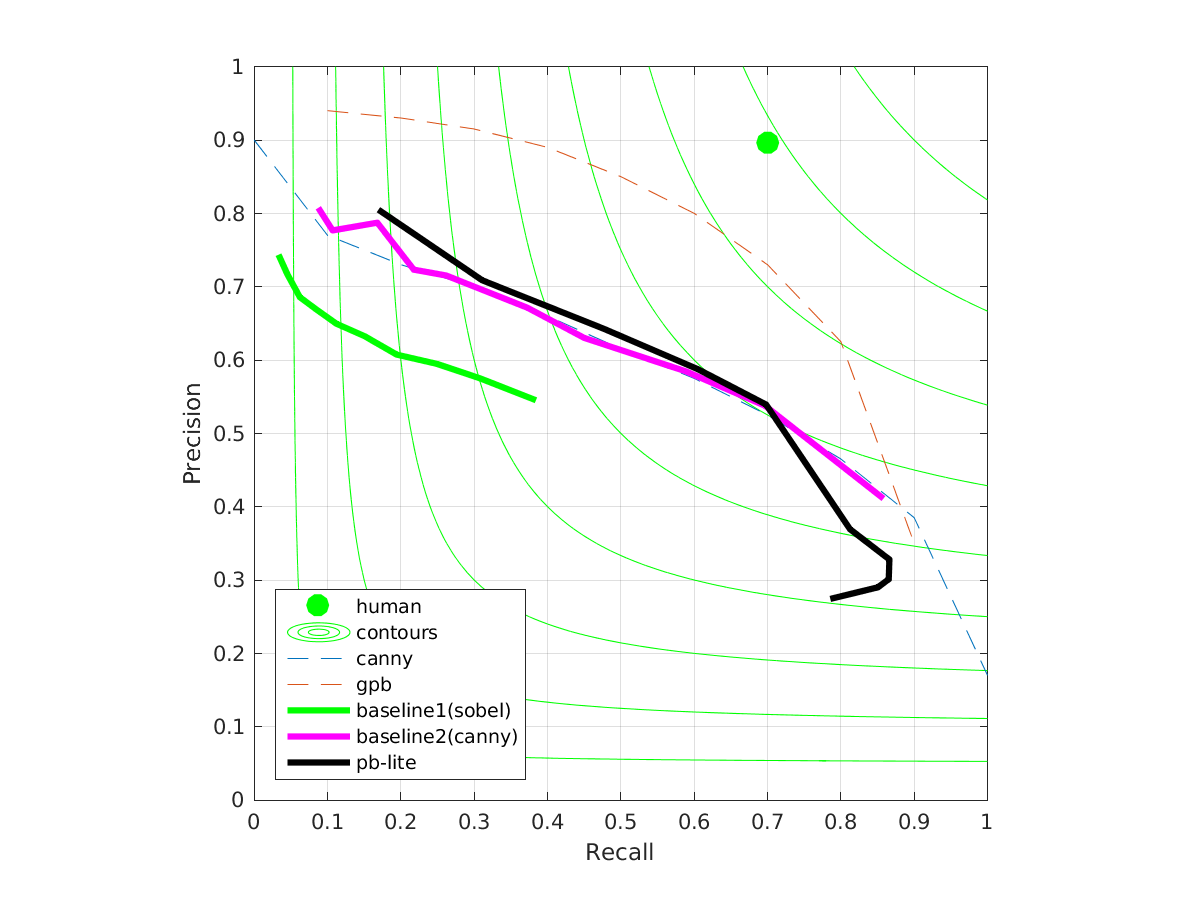
\includegraphics[width=\linewidth]{img/PR_Curve2}
    \caption{My PB result}
    \label{fig_prcurve}
\end{figure}

\begin{figure}
    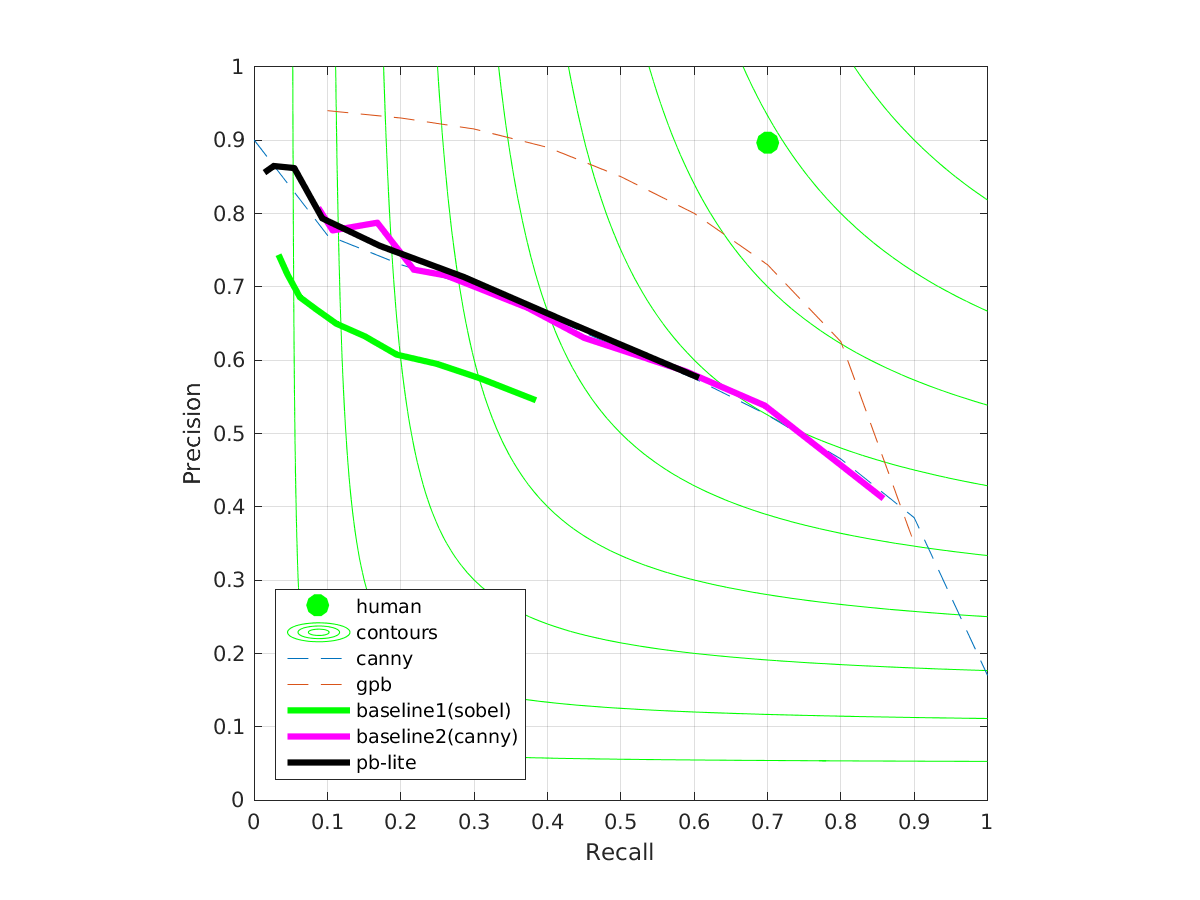
\includegraphics[width=\linewidth]{img/PR_Curve}
    \caption{My result multiplied to canny}
    \label{fig_prcurve}
\end{figure}

\end{document}